\section{Resultados}
O codificador convolucional foi capaz de realizar, em média, a codificação de 1 bit de informação a cada $5.4\mu s$. Para o decodificador, foi possível, em média, realizar decodificação em $84\mu s$, vale ressaltar que o tempo de decodificação varia com o polinômio, no entanto o tempo de codificação não varia com o polinômio e o valor mostrado acima foi um valor médio.

O código foi feito em Python, uma linguagem interpretada, logo, não há arquivo executável. Somando o tamanho de todos os arquivos desenvolvidos durante essa disciplina de laboratório, totaliza-se 100kB. Se forem levados em conta os arquivos das dependências (principalmente numpy e scipy) tem-se um total de 155.5MB. Dessa forma, para executar o projeto desenvolvido como um todo deve-se ter cerca de 160MB disponíveis em disco.

Há um total de vinte grandezas a serem comparadas, o sistema não codificado, o código de Hamming, cinco códigos cíclicos, quatro códigos gerados pela equipe, e nove códigos convolucionais (3 para cada métrica). A fim de tornar a comparação mais fácil, serão exibidos gráficos para cada grupo e um gráfico final comparando um representante de cada grupo. A fim de suavizar as curvas foi utilizado um fit polinomial por meio da função \textit{pchip} do Matlab.

A Figura \ref{fig:cyclic} mostra uma comparação entre todos os códigos cíclicos desenvolvidos.

\begin{figure}[ht]
	\centering
	\captionsetup{justification=centering}
	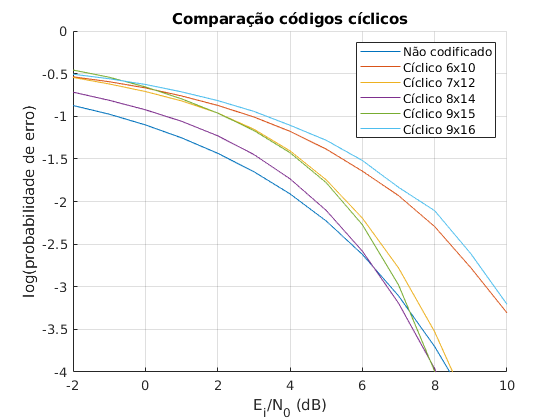
\includegraphics[width=\linewidth]{floats/cyclic.png}
	\caption{\label{fig:cyclic}Comparação da eficácia dos códigos cíclicos para 96768 bits de informação enviados.}
\end{figure}

\newpage
A Figura \ref{fig:proprios} mostra uma comparação entre todos os códigos desenvolvidos pela equipe na primeira prática.

\begin{figure}[ht]
	\centering
	\captionsetup{justification=centering}
	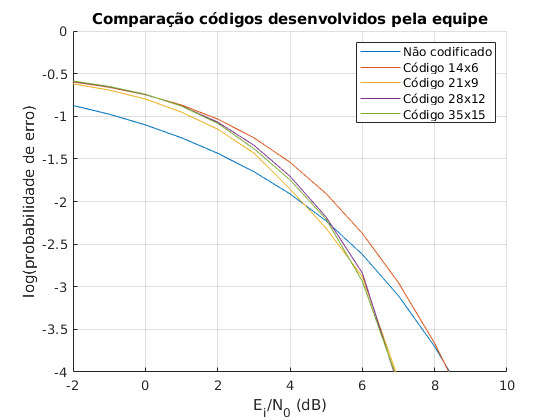
\includegraphics[width=\linewidth]{floats/proprios.png}
	\caption{\label{fig:proprios}Comparação da eficácia dos códigos desenvolvidos pela equipe para 96768 bits de informação enviados.}
\end{figure}

\newpage
As Figuras \ref{fig:convolucionais1}, \ref{fig:convolucionais2}, e \ref{fig:convolucionais3} mostram uma comparação entre todos os códigos convolucionais com as métricas de Hamming, Exata e distância Euclidiana respectivamente. A taxa para todos é $\frac{1}{3}$ e os polinômios utilizados são os do roteiro numerados na ordem em que aparecem no roteiro.

\begin{figure}[ht]
	\centering
	\captionsetup{justification=centering}
	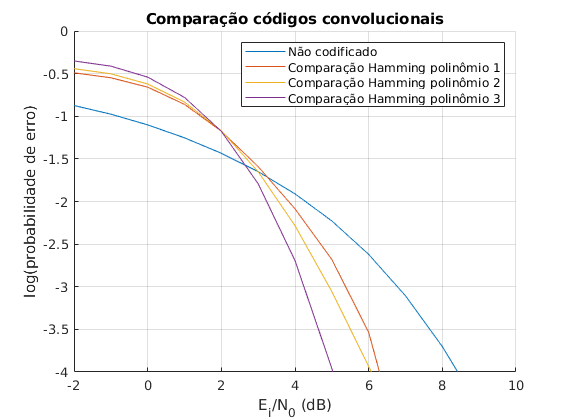
\includegraphics[width=\linewidth]{floats/conv1.png}
	\caption{\label{fig:convolucionais1}Comparação da eficácia dos códigos convolucionais com distância de Hamming para 96768 bits de informação enviados.}
\end{figure}

\begin{figure}[ht]
	\centering
	\captionsetup{justification=centering}
	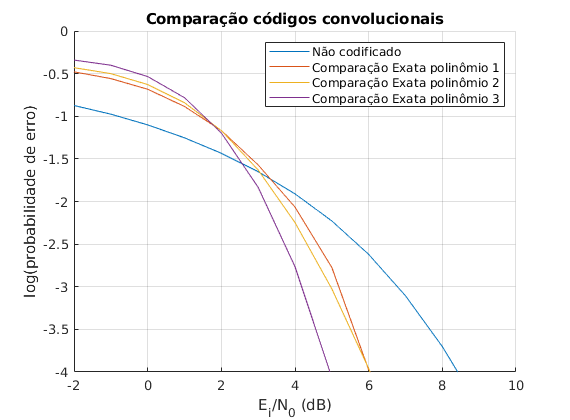
\includegraphics[width=\linewidth]{floats/conv2.png}
	\caption{\label{fig:convolucionais2}Comparação da eficácia dos códigos convolucionais com distância 'Exata' para 96768 bits de informação enviados.}
\end{figure}

\begin{figure}[ht]
	\centering
	\captionsetup{justification=centering}
	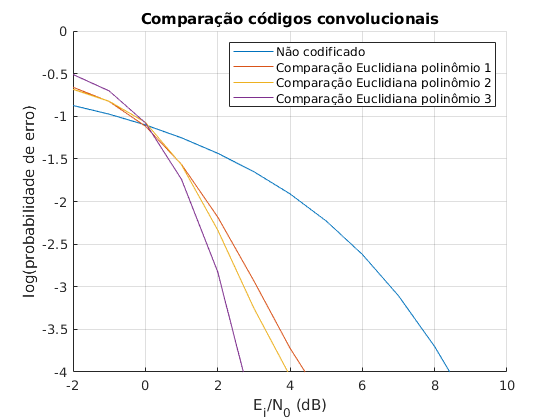
\includegraphics[width=\linewidth]{floats/conv3.png}
	\caption{\label{fig:convolucionais3}Comparação da eficácia dos códigos convolucionais com distância Euclidiana para 96768 bits de informação enviados.}
\end{figure}

\newpage
A Figura \ref{fig:geral} mostra uma comparação entre todos os códigos (é exibido apenas um representante para cada grupo).

\begin{figure}[ht]
	\centering
	\captionsetup{justification=centering}
	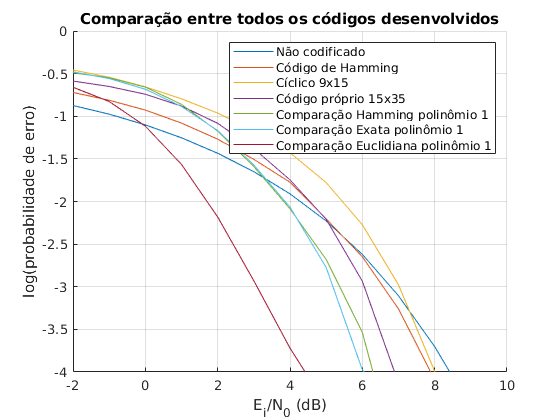
\includegraphics[width=\linewidth]{floats/geral.png}
	\caption{\label{fig:geral}Comparação da eficácia de um representante para cada grupo de códigos para 96768 bits de informação enviados.}
\end{figure}

Para uma taxa de $\frac{1}{3}$ teoricamente o valor de $\frac{E_i}{N_0}$ que permite transmissão com probabilidade de erro zero é de 0.59. Para uma probabilidade de erro de $10^{-4}$ o melhor código convolucional obteve $\frac{E_i}{N_0}$ de 1.86. Isso mostra que o sistema ainda está longe do limite teórico. A Tabela \ref{tab:teorico} mostra tal comparação para cada código analisado.

\begin{table}[h!]
\centering
\caption {Comparação $\frac{E_i}{N_0}$ teórico para probabilidade de erro de transmissão zero e real para probabilidade de erro de transmissão $10^{-4}$} \label{tab:teorico} 
\begin{tabular}{|c|c|c|}
	\hline 
Código analisado	&  Valor teórico de $\frac{E_i}{N_0}$  & Valor real de $\frac{E_i}{N_0}$\\
	\hline 
	Hamming	&  0.81 & 11.0\\ 
	\hline 
	Cíclico 6x10	&  1.30 & 11.0\\ 
	\hline 
	Cíclico 7x12	&  1.25 & 7.1\\ 
	\hline 
	Cíclico 8x14	&  1.20 & 6.3\\ 
	\hline 
	Cíclico 9x15	&  1.30 & 6.3\\ 
	\hline 
	Cíclico 9x16	&  1.18 & 11.5\\ 
	\hline 
	Código próprio 6x14	&  1.20 & 7.0\\ 
	\hline 
	Código próprio 9x21	&  1.20 & 5.0\\ 
	\hline 
	Código próprio 12x28	&  1.20 & 5.0\\ 
	\hline 
	Código próprio 15x35	&  1.20 & 5.0\\ 
	\hline 
	Código conv Hamming pol1	&  0.59 & 4.22\\ 
	\hline 
	Código conv Hamming pol2	&  0.59 & 3.98\\ 
	\hline 
	Código conv Hamming pol3	&  0.59 & 3.16\\ 
	\hline
	Código conv Exact pol1	&  0.59 & 3.98\\ 
	\hline 
	Código conv Exact pol2	&  0.59 & 3.98\\ 
	\hline 
	Código conv Exact pol3	&  0.59 & 3.10\\ 
	\hline
	Código conv Euclidean pol1	&  0.59 & 2.66\\ 
	\hline 
	Código conv Euclidean pol2	&  0.59 & 2.51\\ 
	\hline 
	Código conv Euclidean pol3	&  0.59 & 1.86\\ 
	\hline
	
\end{tabular} 

\end{table}
\newpage